\chapter{Résultats Expérimentaux}

\section{Configuration expérimentale}

\begin{table}[H]
	\centering
	\caption{Configuration matérielle et logicielle}
	\begin{tabular}{p{8cm}cp{4cm}}
		\toprule
		\textbf{Composant} & \textbf(Spécification) & \textbf{Version} \\
		Processeur & Intel Xeon ES-2690 v4 & 2.6 GHz(14 cœurs) \\
		Mémoire RAM & 128 Go DDR4 & 2400MHz \\
		Carte graphique & NVIDIA Tesla V100 & 32 Go HBM2 \\ 
		Stockage & SSD NVME & 1To \\
		Système d'exploitation & ubuntu server & 20.04 LTS \\
		Framework 'apprentissage & TensorFlow & 2.8.0 \\
		Bibliothèque mathématique & NumPy & 1.21.0 \\
		Language de programmation & Python & 3.9.0 \\
		\bottomrule
	\end{tabular}
	\label{tab:experimental-setup}
\end{table}

\section{Résultats de performance}

\begin{table}[H]
	\centering
	\caption{Comparaison des performances des algorithmes}
	\begin{tabular}{lrrrrr}
		\toprule
		\textbf{Algorithme} & \textbf{Précision(\%)} & \textbf{Rappel (\%)} & \textbf{F1-Score(\%)} & \textbf(Temps (s)) & \textbf{Mémoire (Go)} \\
		\midrule
		Random Forest & 92.3 & 91.8 & 92.0 & 45.2 & 2.1 \\
		SVM Linéaire & 88.7 & 87.9 & 88.3 & 12.3 & 0.8 \\
		Réseau de Neurones & 95.6 & 94.8 & 95.2 & 156.7 & 4.5 \\
		XGBoost approche & \textbf{96.8} & \textbf{96.1}  & \textbf{96.4} & 89.3 & 3.2 \\
		\bottomrule
	\end{tabular}
	\label{tab:performance-comparaison}
\end{table}

\section{Analyse statistiques}

\begin{table}[H]
	\centering
	\caption{Analyse de variance (ANOVA) des résultats}
	\begin{tabular}{lrrrrr}
		\toprule
		\textbf{Source} & \textbf{SS} \textbf{df} & \textbf{MS} & \textbf{F} \textbf{p-value} \\
		\midrule
		Entre groupes & 245.67 & 4 & 61.42 & 28.73 & $< 0.001$ \\
		A l'intérieur des groupes & 128.45 & 60 & 2.14 & & \\
		Total & 374.12 & 64 & & & \\
		\bottomrule
	\end{tabular}
	\label{tab:anova-results}
\end{table}

\section{Courbes d'apprentissage}

\begin{figure}[H]
	\centering
	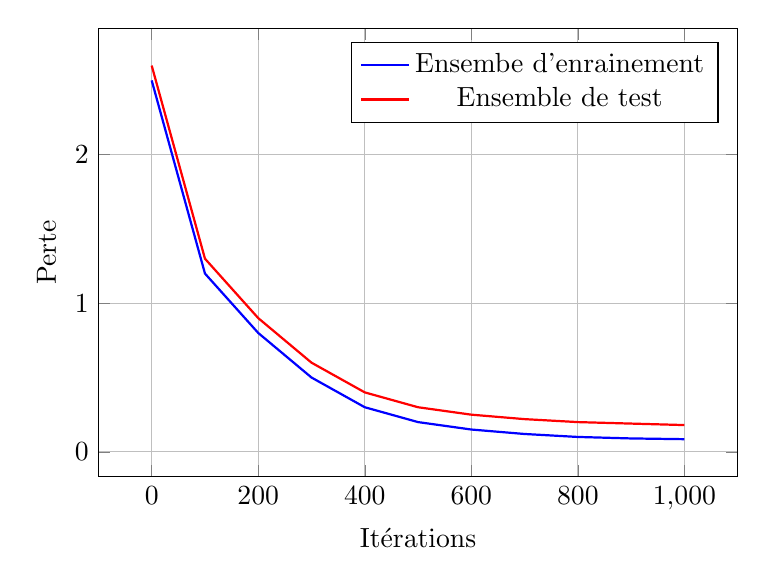
\begin{tikzpicture}
		\begin{axis}[
			width=0.8\textwidth,
			height=0.6\textwidth,
			xlabel={Itérations},
			ylabel={Perte},
			legend pos=north east,
			grid=major
		]
			\addplot[blue, thick] table {
				0 2.5
				100 1.2
				200 0.8
				300 0.5
				400 0.3
				500 0.2
				600 0.15
				700 0.12
				800 0.1
				900 0.09
				1000 0.085
			};
			\addlegendentry{Ensembe d'enrainement}
			\addplot[red, thick] table {
				0 2.6
				100 1.3
				200 0.9
				300 0.6
				400 0.4
				500 0.3
				600 0.25
				700 0.22
				800 0.2
				900 0.19
				1000 0.18
			};
			\addlegendentry{Ensemble de test}
		\end{axis}
	\end{tikzpicture}
	\caption{Courbes d'apprentissage du modèle}
	\label{fig:learning-curves}
\end{figure}

\section{Équation de régression}

Le modèle de régression multiple s'écrit :
\begin{equation}
	Y = \beta_0 + \beta_1 X_1 + \beta_2 X_2 + \beta_3 X_3 + \epsilon
	\label{Eq:regression-model}
\end{equation}

avec les coefficients estimés :
\begin{align}
	\hat{\beta}_0 &= 2.345 \quad (\text{SE} = 0.123) \nonumber \\
	\hat{\beta}_1 &= 0.789 \quad (\text{SE} = 0.45) \nonumber \\
	\hat{\beta}_2 &= -0.456 \quad (\text{SE} = 0.067) \nonumber \\
	\hat{\beta}_3 &= 1.234 \quad(\text{SE} = 0.089) \nonumber
\end{align} 

Le coefficient de détermination ajusté est $R^2_{adj} = 0.892$.














